\section{Normal Distribution}

The normal distribution is the most important continuous distribution in statistics and appears in the \emph{Central Limit Theorem}.

\begin{definicion}[Normal Distribution]
A continuous random variable $X$ has a \emph{normal distribution} with parameters $\mu$ (mean) and $\sigma > 0$ (standard deviation) if its density function is
\begin{align}
 \label{eq:2.8.3}
 f(x) = \frac{1}{\sigma\sqrt{2\pi}}\,\exp\!\left(-\frac{(x-\mu)^2}{2\sigma^2}\right),
 \qquad x \in \mathbb{R}.
\end{align}
We write $X \sim N(\mu, \sigma^2)$.
\end{definicion}

{Properties of the normal distribution} If $X \sim N(\mu,\sigma^2)$, then
\begin{itemize}
 \item The distribution is \emph{symmetric} with respect to $\mu$.
 \item $\mu$ is the mean, median, and mode.
 \item $\sigma^2$ is the variance.
 \item If $Z \sim N(0,1)$ (standard form), then $X = \mu + \sigma Z$.
\end{itemize}

{Standard form} If $X \sim N(\mu, \sigma^2)$, the standardized variable
\begin{align}
 \label{eq:2.8.4}
 Z = \frac{X - \mu}{\sigma}
\end{align}
follows an $N(0,1)$ distribution with density
\begin{align}
 \label{eq:2.8.5}
 \varphi(z) = \frac{1}{\sqrt{2\pi}}\,e^{-z^2/2}, \qquad z \in \mathbb{R}.
\end{align}

{Empirical Rule $68$--$95$--$99.7$} If $X \sim N(\mu,\sigma^2)$, then
\begin{align}
 P(\mu - \sigma \leq X \leq \mu + \sigma) &\approx 0.6827, \\
 P(\mu - 2\sigma \leq X \leq \mu + 2\sigma) &\approx 0.9545, \\
 P(\mu - 3\sigma \leq X \leq \mu + 3\sigma) &\approx 0.9973.
\end{align}

\begin{observacion}
The normal distribution appears in many practical situations: measurement errors, human heights, test scores, etc. Furthermore, by the Central Limit Theorem, the sum (or average) of many independent random variables (under mild conditions) is approximately normal.
\end{observacion}

\begin{ejemplo}
 \label{exmp:2.8.2}
The scores on an exam follow an $N(70, 100)$ distribution (mean $70$, variance $100$, i.e., $\sigma=10$). What percentage of students scored between $60$ and $80$ points?
\end{ejemplo}

\begin{solucion}
We standardize: if $X \sim N(70, 100)$, then
\begin{align}
 P(60 \leq X \leq 80) = P\!\left(\frac{60-70}{10} \leq Z \leq \frac{80-70}{10}\right)
 = P(-1 \leq Z \leq 1).
\end{align}

By the empirical rule, this value is approximately $0.6827 = 68.27\%$. Using tables or software, the exact value is $\Phi(1) - \Phi(-1) = 0.8413 - 0.1587 = 0.6827$.
\end{solucion}

\lstinputlisting[language=Python]{../code/distribuciones-continuas-avanzadas/distNormalContinua.py}

\begin{figure}
 \centering
 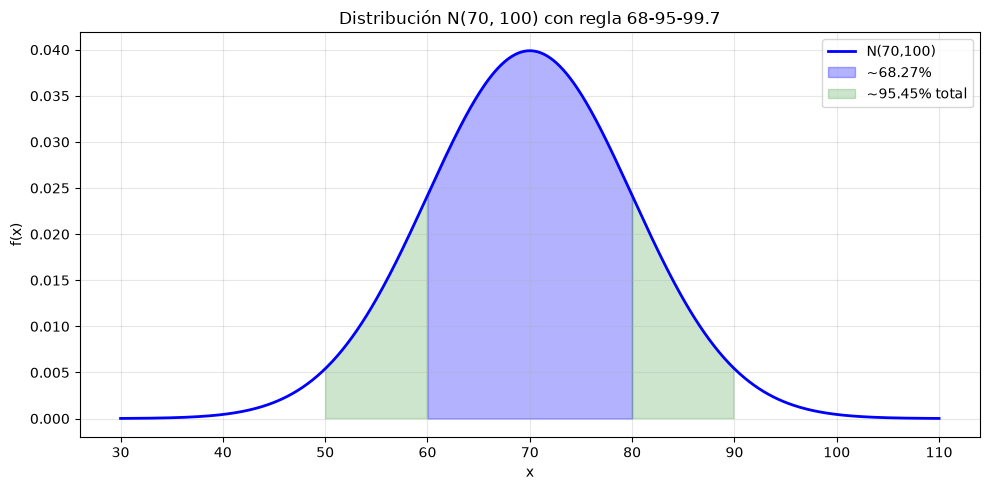
\includegraphics[height=7cm,keepaspectratio=true]{./pe/distNormalContinua.png}
 % distNormalContinua.png: 0x0 pixel, 300dpi, 0.00x0.00 cm, bb=
 \caption{Distribution $N(70,100)$ illustrating the 68--95--99.7 empirical rule.}
 \label{fig:2.8.2}
\end{figure}
